\section{Rash model}
\label{sec:eval-rasch}

\subsection{Goals and research questions}
The main \textit{goal} of the first experiment is to discover correlations between the difficulty of an exercise as estimated by the \gls{2pl} model, and characteristics of that exercise.
The \textit{purpose} is to gain insights in the mental model of the developer, and discover which languages, frameworks, or vulnerability types are typically more difficult.
The results of this experiment can be used in the \gls{its} to approximate the difficulty of an exercise when there is no sufficient data available to obtain an estimate with \gls{irt}.

The above goal can be achieved by means of an experiment aimed at answering the following questions:
Is there a statistically significant correlation between the difficulty of a challenge and its
\begin{itemize}
    \item \textbf{Q1} assigned difficulty on the \gls{scw} platform?
    \item \textbf{Q2} vulnerability category?
    \item \textbf{Q3} vulnerability type (subcategory)?
    \item \textbf{Q4} language and framework?
    \item \textbf{Q5} presentation form (locate, identify, fix)?
\end{itemize}

It is expected that the last four characteristics have a significant influence on the difficulty of a challenge.
Some vulnerabilities are more difficult to detect, understand, or fix than others.
This is evident, for example, from the \gls{owasp} Top 10 pages, where each category is assigned a score for exploitability, prevalance, detectability, and technical impact.
There is no clear explanation as to how these scores are determined.
Personal and anecdotal evidence also shows that it is more difficult to get security right while working in certain languages and frameworks.

The first variable, the assigned difficulty on the \gls{scw} platform, is expected to have little impact on the actual difficulty.
As explained in Appendix~\ref{app:challenges}, this difficulty only represents the probability of a correct answer in case of a blind guess.
It does not take into account the contents of the exercise, only the number of options to choose from.
While the amount of options is expected to have some influence on the actual difficulty, this effect is likely to be small compared to other characteristics of the exercise.

\subsection{Experimental set-up}
In Section~\ref{sec:calib}, it was previously mentioned that calibration techniques for the \gls{2pl} model are mostly designed for item banks with several dozens of items.
The larger size of the item bank of \gls{scw} will cause longer execution times and more difficult convergence to stable estimates.
I solved this problem by splitting the item bank into several smaller item banks and calibrating each of them separately.

The downside to this approach is that the \gls{2pl} model does not use an absolute scale.
This is evident from the equation for the \gls{1pl} model in Equation~\ref{eq:1pl}, repeated here for convenience in Equation~\ref{eq:1pl-2}.

\begin{equation}
    \label{eq:1pl-2}
    P_{j}(\bm{\theta}_i,\bm{p}_j) =
    Pr(X_{ij} = 1 | \bm{\theta}_i,b_j) =
    \frac{\exp(\theta_i - b_j)}{1 + \exp(\theta_i - b_j)}
\end{equation}

Adding or subtracting the same value from both the difficulty parameter $b_j$ and the ability level $\theta_i$ will cancel out and result in the same probability of a correct answer $P_j$.
In other words, the origin of the scale can be chosen arbitrarily.
In practice, the origin is often set to the mean of the ability estimates~\cite{magis2017computerized}.
I used the R package \texttt{TAM} to estimate the item and person parameters~\cite{robitzsch2021package}.
In the documentation of this package there is no information about the chosen scale.
Based on the implementation that is available on GitHub\footnote{\url{https://github.com/cran/TAM/blob/master/R/tam.mml.2pl.R}}, the scale is set to the mean of the difficulty estimates after the first iteration of the calibration process.
For each item bank that is calibrated separately, the results can hence not be easily compared to other item banks, as they each have their own scale.

However, for this experiment it is necessary to compare the difficulty of challenges across the entire platform.
To be able to do this, the entire item bank has to be calibrated at once. 
The necessary computations took over 73 hours to complete, confirming once more that it would not be feasible to use in the \gls{its}.

% TODO:
% MacBook Pro (16-inch 2019)
% Intel(R) Core(TM) i9-9980HK CPU @ 2.40GHz
% 32 GB DDR4 dual channel memory @ 2667 MHz

\subsubsection{Statistical significance}
With this single \gls{2pl} model calibrated, there is a difficulty estimate for every challenge on the platform.
It is now possible to group these challenges according to different characteristics and compute the mean difficulty of each group.
Before we can compare the mean difficulties for each characteristic, however, the results have to be tested for statistical significance.

Which test can be used to do this, depends on the values each characteristic can take.
The difficulty as assigned on the \gls{scw} platform takes on values between 0 and 100, and is hence a numerical variable.
The vulnerability category, vulnerability type, framework, and presentation form are each categorical variables.
Each of these characteristics can only take a limited number of categorical values.

To test the correlation between the difficulty on the \gls{scw} training platform and the \gls{irt} difficulty, the coefficient of determination (R-squared) can be used, as both variables are numerical variables.
The test (R = 0.03, $p = 1.85 \times 10^{-3}$) determines that no significant variation in the \gls{irt} difficulty can be explained by the \gls{scw} difficulty.
This is no surprise, it is clear that the current difficulty assigned on the platform is not an accurate representation of the actual difficulty.

A one-way \gls{anova} can be used for the categorical variables.
This test determines if there is a statistically significant difference between one or more of the possible values that a categorical variable can take.
The one-way \gls{anova} compares the mean difficulty for each of those values and determines whether any of those means are statistically significantly different from each other.
If the one-way \gls{anova} returns a statistically significant result, that means there are at least two values that are statistically different from each other.

The variables were found to have unequal variances across the possible values, a property called heterogeneity of variances.
A Welch \gls{anova} should hence be used, as this \gls{anova} can account for type I errors~\cite{liu2015comparing}.
The results of the Welch \glspl{anova} are shown in Table~\ref{tab:anova1} and show that a statistically significant difference exists between values for each of the categorical variables.

\begin{table}
    \centering
    \caption[\Gls{anova} test results for 2PL model]{The results of one-way \gls{anova} tests between variables of the exercises and the estimated difficulty. For each variable, the degrees of freedom (df) are shown, as well as the F-statistic, the $p$-value, and the eta-squared ($\eta^2$). All four categorical variables have statistically significant correlations with the estimated difficulty of the exercise. The presentation has a large effect on the estimated difficulty. The category, vulnerability, and framework each have a medium effect.}
    \setcellgapes{4pt}\makegapedcells
    \begin{tabular}{l l S[table-format=3.3] l l}
Variable & df & F & $p$ & $\eta^2$ \\
    \hline
    Category & 36 & 14.154 & $2.97 \times 10^{-53}$ & 0.046 \\
    Vulnerability & 142 & 5.393 & $1.19 \times 10^{-45}$ & 0.079 \\
    Framework & 38 & 11.430 & $ 1.49 \times 10^{-41}$ & 0.060 \\
    Presentation & 3 & 346.164 & $3.00 \times 10^{-6}$ & 0.155 \\
    \end{tabular}
    \label{tab:anova1}
\end{table}

In this \gls{anova}, the eta-squared ($\eta^2$) metric was used to measure the effect size of each categorical variable on the estimated \gls{irt} difficulty.
A medium effect was measured for the framework, category, and vulnerability of the exercise and a large effect was measured for the presentation.

Pairwise Games-Howell post-hoc tests were then used to determine which of the values in each categorical variable are statistically different from each other~\cite{games1976pairwise}.
Results of these tests are shown in Table~\ref{tab:gameshowell}.

\begin{table}
    \centering
    \caption[Pairwise Games-Howell post-hoc test results]{The second column displays the number of possible values. Every one of those values is paired with all other values for a pairwise Games-Howell test. The next two columns report the amount of pairs for which the means differ in a statistically significant way, and the amount of pairs for which this is not the case. In the final column the number of values is shown, for which at least one pair exists where the means are statistically significantly different.}
    \setcellgapes{4pt}\makegapedcells
    \renewcommand\theadfont{\normalsize}
    \begin{tabular}{l l l l l}
    Variable & \thead{Values} & \thead{Significant\\ pairs} & \thead{Insignificant\\ pairs} & \thead{Significant\\ values} \\
    \hline
    Category & 36 & 118 & 548 & 29 \\
    Vulnerability & 142 & 384 & 9769 & 77 \\
    Framework & 38 & 217 & 524 & 37 \\
    Presentation & 3 & 3 & 0 & 3 \\
    \end{tabular}
    \label{tab:gameshowell}
\end{table}


With the exception of the presentation, each of the categorical variables has a number of values that do not show a statistical significance with any other value.
If there is no statistical significant difference between two values, this is usually due to insufficient data for one of the values or because the data of one (or both) of the values is too widely spread and there is significant overlap between the data for the two values.
%In the remainder of this section such values are not discussed or shown in any of the graphical displays.
The remaining values show a statistically significant difference in mean difficulty with at least one other value.
When mean difficulties are compared in the remainder of this chapter, only values are compared whose means show statistically significant differences as determined by the pairwise Games-Howell tests.
Each of the values that are compared explicitly, show statistically significant differences in mean difficulty with a $p$-value of at most 0.05.
The exact $p$-values of these tests are reported in Appendix~\ref{app:pairups}.
%Where appropriate, the $p$-values of the pairwise Games-Howell test for compared categories will be included.

\subsection{Findings}
In this section, I report some of the notable differences in difficulty between different values for each of the characteristics and offer possible explanations for these observations.

\subsubsection{Vulnerability category}
There is a statistically significant difference between the mean difficulty of the four hardest and the four easiest categories.
When comparing these categories to each other, as shown in Figure~\ref{fig:cats1}, their difficulty seems mostly related to the locality of the vulnerability type.

\begin{figure}
    \centering
    %\input{03-education/plots/categories}
    \includegraphics[page=20]{03-education/figures/tikzfigures.pdf}
    \caption[Difficulty of bugs versus flaws]{Vulnerabilities that often require only local changes to the code to fix have lower mean difficulties.}
    \label{fig:cats1}
\end{figure}

The top four categories are (design) \glspl{flaw}, and the fix often involves larger pieces of code.
This is especially the case for business logic flaws and denial of service, where the complexity of the code is the main cause of the problem.
In these categories the developer is unable to foresee unintended results that are a direct result of the logic of their code.
%Some examples are logical errors, uncaught error handling, and problems with regular expressions.

The fixes of the four easiest categories usually only require local changes to the code.
Injection and \gls{xxe} are often fixed by properly sanitizing or whitelisting input parameters, or by configuring components properly.
Security problems related to session management are things like incorrect session lengths, insufficient entropy, or insufficient length for the session \glspl{id}.
Use of vulnerable components is most frequently fixed by updating to a version of the component where the vulnerabilities are fixed.
To fix these vulnerabilities, only local changes to the code are necessary, identifying the correct fix out of several options only involves building a mental model of a small piece of code, making it easier to reason about.

Still, it is noteworthy that the categories near the bottom of the scale are some of the most infamous vulnerabilities.
Injection for example is the top category of the \gls{owasp} top 10 in 2017 and receives high scores for exploitability, detectability, and technicality.
It has currently dropped to the third position in the iteration released in 2021\footnote{\url{https://owasp.org/Top10/}}.
Based on our training data, at least, it seems that these scores might be exaggerated.
%To explain this, we have to consider the exercises on the \gls{scw} platform.
%To locate a vulnerability in the code, the category of the vulnerability is given.
%At the same time, these vulnerabilities are related to very specific pieces of code. \gls{sql} injection for example can only occur in database queries.
%This makes locating the vulnerability easier.
One exception to this is \gls{xss}.
Despite its infamy, it is closer to the middle of the scale, as can be seen in Figure~\ref{fig:cats2} where \gls{xss} is shown together with all categories it shows statistically significant differences with.
\Gls{xss} being in the middle of the scale can be explained by the fact that there are two major types of \gls{xss}, stored \gls{xss} and reflected \gls{xss}. 
In the case of reflected \gls{xss} the vulnerability is rather local, and the fix is also applied locally, by using output encoding.
For stored \gls{xss} there are usually multiple code fragments involved, one or more where the user input is stored as data and one or more where the stored data is used without output encoding.

In conclusion, the difficulty of the vulnerability correlates to the size of the related code fragments.
Vulnerabilities that only require local changes in the code to fix are easier to understand and fix in training, despite their apparent prevalence in practice.

\begin{figure}
    \centering
    %\input{03-education/plots/categories}
    \includegraphics[page=21]{03-education/figures/tikzfigures.pdf}
    \caption[Medium mean difficulty for XSS challenges]{Challenges about XSS show a mean difficulty around the middle of the scale.}
    \label{fig:cats2}
\end{figure}

\subsubsection{Framework}
Of the 38 different frameworks, 37 show statistically significant differences with at least one other framework.
Pseudocode shows a significant difference with 17 of these frameworks, all of which have a higher mean difficulty.
This makes sense as pseudocode is an artificial language.
It is designed to teach developers algorithms and other programming concepts, and should be easy to understand.

Memory management in memory-unsafe languages such as C and C++ can lead to a whole class of security problems that are avoided in memory-safe languages.
We can see this effect in the higher mean difficulty of C and C++ compared to those of the modern, memory-safe programming languages Java, C\# (.NET), and Python, as shown in Figure~\ref{fig:frames1}.
However, the memory-safe language Cobol also shows a statistically significantly higher mean difficulty compared to each of these three languages.
While Cobol is memory-safe, it does still require memory management and use of pointers, which might explain the higher mean difficulty.
Cobol is also known for its lack of clear documentation regarding security concepts.

\begin{figure}
    \centering
    %\input{03-education/plots/frameworks1}
    \includegraphics[page=9]{03-education/figures/tikzfigures.pdf}
    \caption[Memory-safe versus memory-unsafe languages]{Older programming languages require memory management and use of pointers. They show harder mean difficulties than languages that have automated memory management.}
    \label{fig:frames1}
\end{figure}

Several frameworks show statistically significant differences between the framework and its standard programming language.
This is the case for Java Spring, Java \gls{ee}, Java \gls{jsf}, C\# (.NET) Web Forms, and Python Django.
All of these frameworks are more difficult than their standard language counterparts, as shown in Figure~\ref{fig:frames2}.
This is surprising, as frameworks are designed to implement commonly used functions so that the developer does not have to.
For example, to securely hash a password in standard Java, the developer has to research which algorithm is the most secure, they have to generate a salt using a secure random number generator and correctly combine each of these techniques.
In Java Spring a \texttt{PasswordEncoder} interface is provided, the documentation of this interface is brief and informs developers that \texttt{BCryptPasswordEncoder} is the preferred implementation\footnote{\url{https://docs.spring.io/}}.

Because frameworks often automate these commonly used features, some details of the implementations might be lost to developers.
This is also confirmed by previous research where 44\% of analyzed applications were shown to contain vulnerabilities caused by misunderstandings of the framework implementation details~\cite{votipka2020understanding}.
When the implementation in such a framework is insufficient, or when the framework is used incorrectly, it is possible that even a security conscious developer can remain unaware of the consequences.
On top of the standard language skills, and the security knowledge, a developer using a framework hence also needs an intimate knowledge of the framework itself to deliver secure code.

\begin{figure}
    \centering
    %\input{03-education/plots/frameworks2}
    \includegraphics[page=10]{03-education/figures/tikzfigures.pdf}
    \caption[Frameworks versus default languages]{All of the frameworks that show statistically significant differences with their standard programming language, have a higher mean difficulty.}
    \label{fig:frames2}
\end{figure}

The mobile framework Java Android is more difficult than web frameworks for the same language (Java \gls{jsf}, Java Spring), as shown in Figure~\ref{fig:frames3}.
This can be explained through the increased attack vectors of mobile applications that are installed on the device of the user.
Because the device and operating system cannot be trusted, the developer has to be aware of other threats, such as restoring backups that are tampered with, detecting root access, and tapjacking, a vulnerability where the attacker can trick the user to perform unintended actions by drawing overlays.
Unfortunately, Objective C, an extension of C that can be used for mobile development, does not show a statistically significant difference with C itself to confirm this correlation.
The more modern replacement for Objective C, Swift, that is inspired by both C\# (.NET) and Python does show a statistically significant higher mean difficulty than both these languages~\cite{nondot}.

Languages and frameworks have evolved to automate some of the tasks of the developer, such as memory management, and password encryption.
The abstractions provided by these languages and frameworks do not always have a positive impact on security, as is evident from these results.
It is likely that the developer has to sufficiently grasp the implementation details to fully understand the security impact of their code.

\begin{figure}
    \centering
    %\input{03-education/plots/frameworks3}
    \includegraphics[page=11]{03-education/figures/tikzfigures.pdf}
    \caption[Mobile versus web frameworks]{Mobile framework and languages that show statistically significant differences with their web counterparts have higher mean difficulties.}
    \label{fig:frames3}
\end{figure}

\subsubsection{Presentation}
A challenge can be presented to the user as an identify, locate, or fix exercise.
It is unsurprising that identifying a vulnerability that is already marked in the code, is the easiest type of exercise, as shown in Figure~\ref{fig:presentation}. 
On the platform this type of exercise is usually the first stage of a two-stage challenge, with the second stage a fix exercise.

\begin{figure}
    \centering
    %\input{03-education/plots/frameworks3}
    \includegraphics[page=22]{03-education/figures/tikzfigures.pdf}
    \caption[Mean difficulty of challenge presentation]{The mean difficulty of each presentation form is statistically different of the other two. In line with observations in practice, locating a vulnerability in code is the most difficult of the three tasks, followed by fixing the vulnerability.}
    \label{fig:presentation}
\end{figure}

According to the \gls{2pl} model, locating vulnerabilities in the code is the most difficult task.
This is in line with observations made in practice, where many vulnerabilities go unnoticed by developers and are detected by automated tools at later stages in the \gls{sdlc}.